\documentclass[12pt]{article}
\usepackage{amsmath}
\usepackage{array}
% \usepackage{gensymb}
\usepackage{geometry}
\usepackage{graphicx}
\usepackage{pgfplots}
\usepackage{siunitx}
\usepackage{wrapfig}

\title{Homework \#2, 4B}
\author{Donald Aingworth IV}
\date{January 29, 2025}

\pgfplotsset{width=8cm,compat=1.9}
\usepgfplotslibrary{external}
% \tikzexternalize

\begin{document}

\DeclareSIUnit{\mile}{mi}
\DeclareSIUnit{\gal}{gal}
\DeclareSIUnit{\foot}{ft}
\DeclareSIUnit{\hour}{h}
\DeclareSIUnit{\rad}{rad}
\DeclareSIUnit{\unit}{u}
\DeclareSIUnit{\dyne}{dyn}

\maketitle

\pagebreak
\section*{Chapter 21, Problem 52}
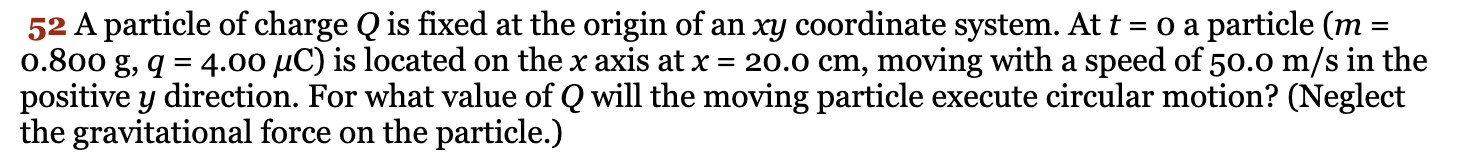
\includegraphics[width=\textwidth]{picture_1.png}


\pagebreak
\section*{Chapter 21, Problem 66}
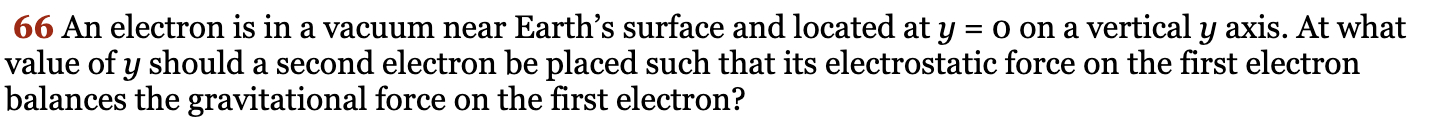
\includegraphics[width=\textwidth]{picture_2.png}


\pagebreak
\section*{Chapter 22, Question 4}
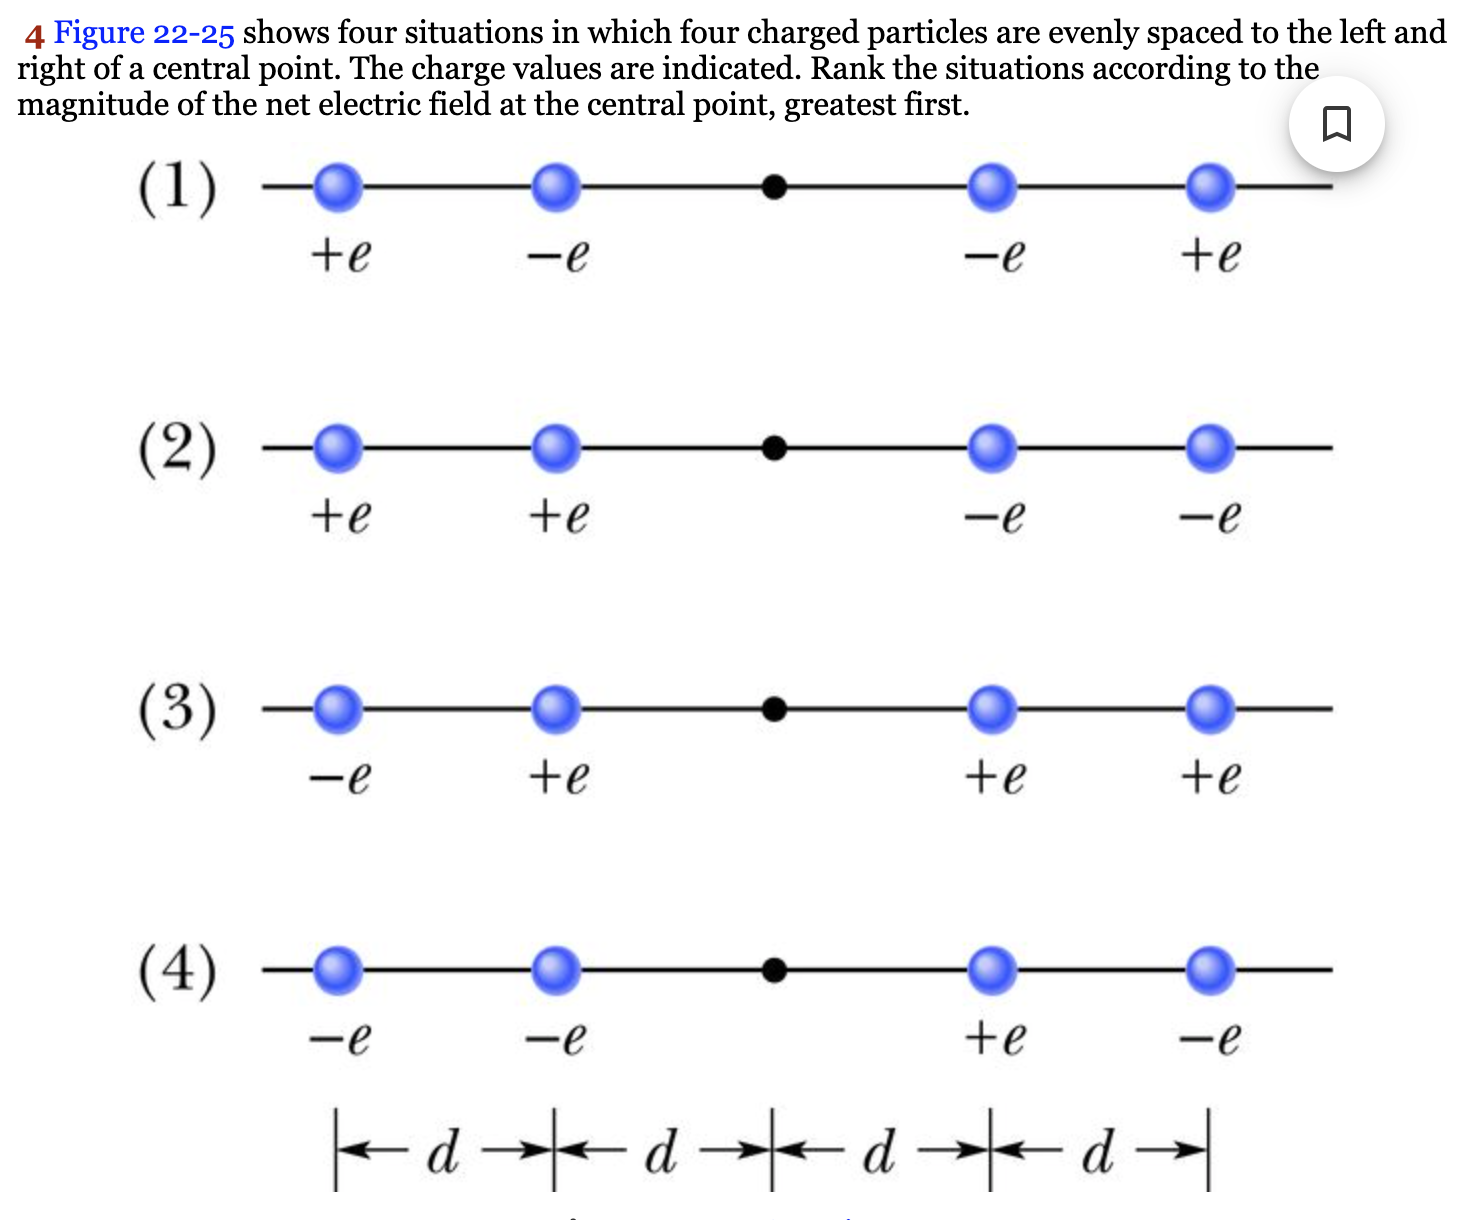
\includegraphics[width=\textwidth]{picture_3.png}


\pagebreak
\section*{Chapter 22, Question 5}
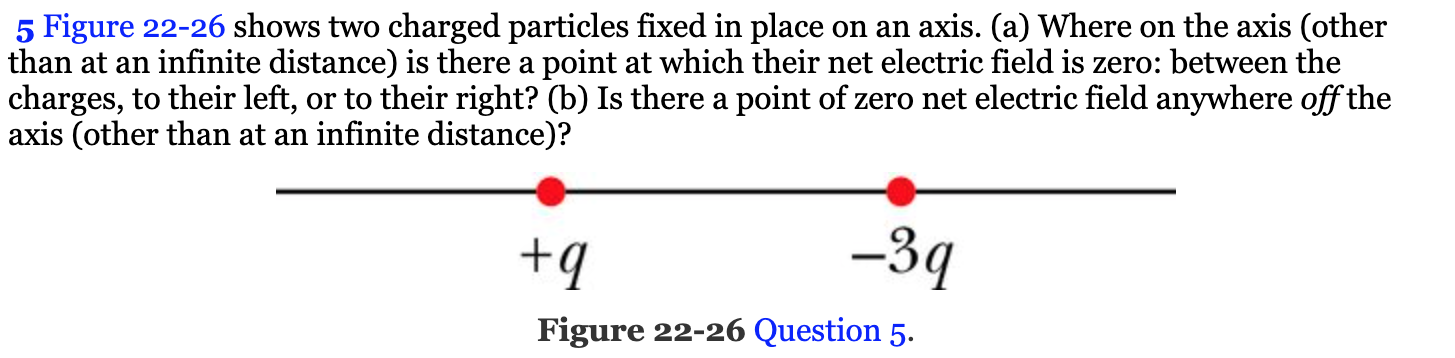
\includegraphics[width=\textwidth]{picture_4.png}


\pagebreak
\section*{Chapter 22, Problem 8}
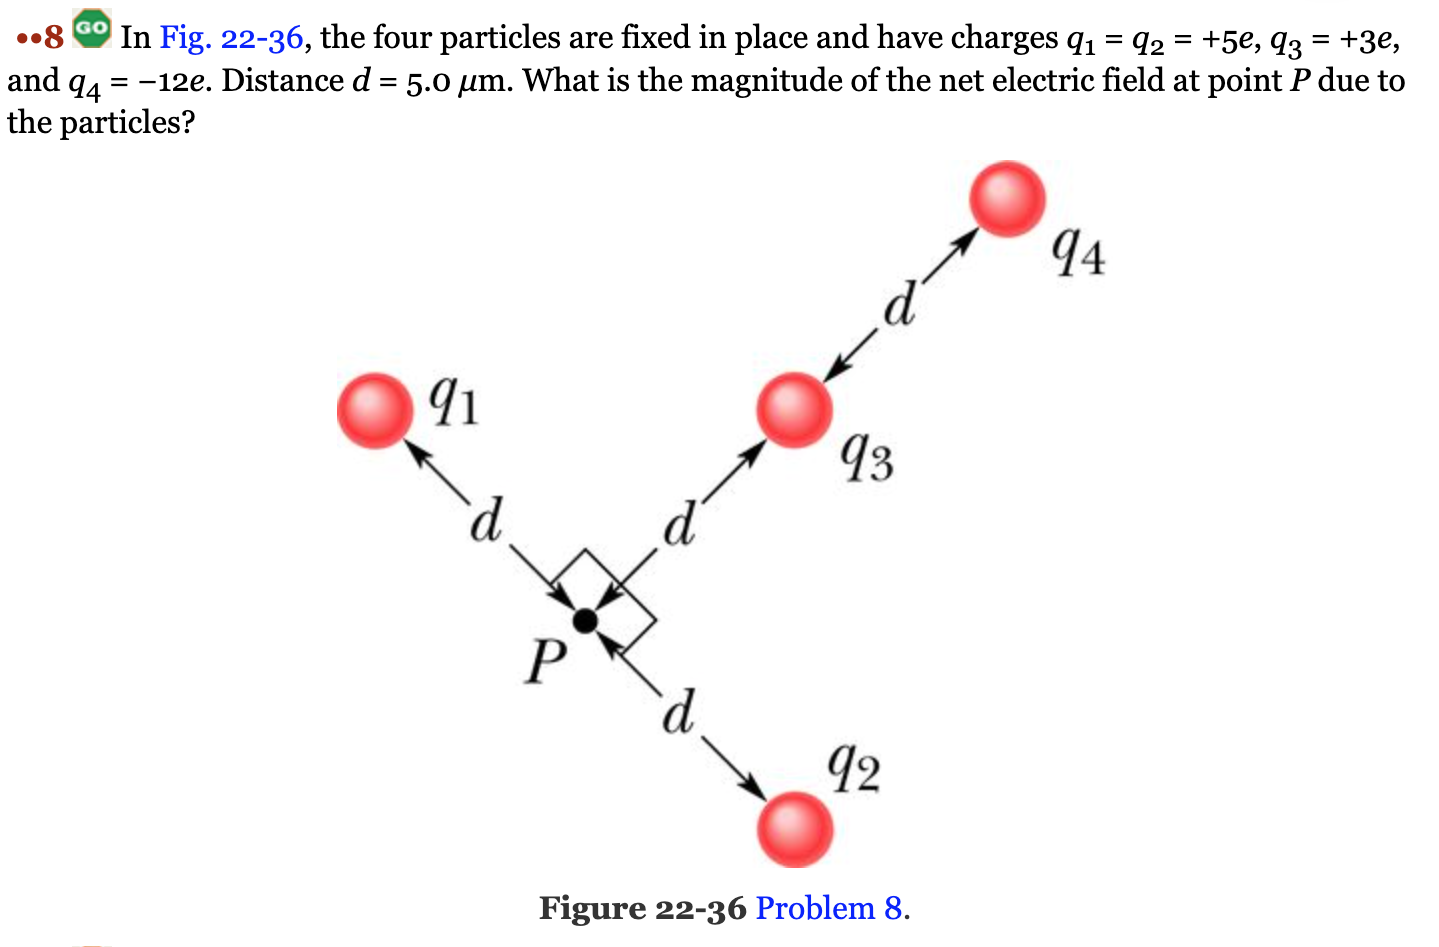
\includegraphics[width=\textwidth]{picture_5.png}


\pagebreak
\section*{Chapter 22, Problem 12}
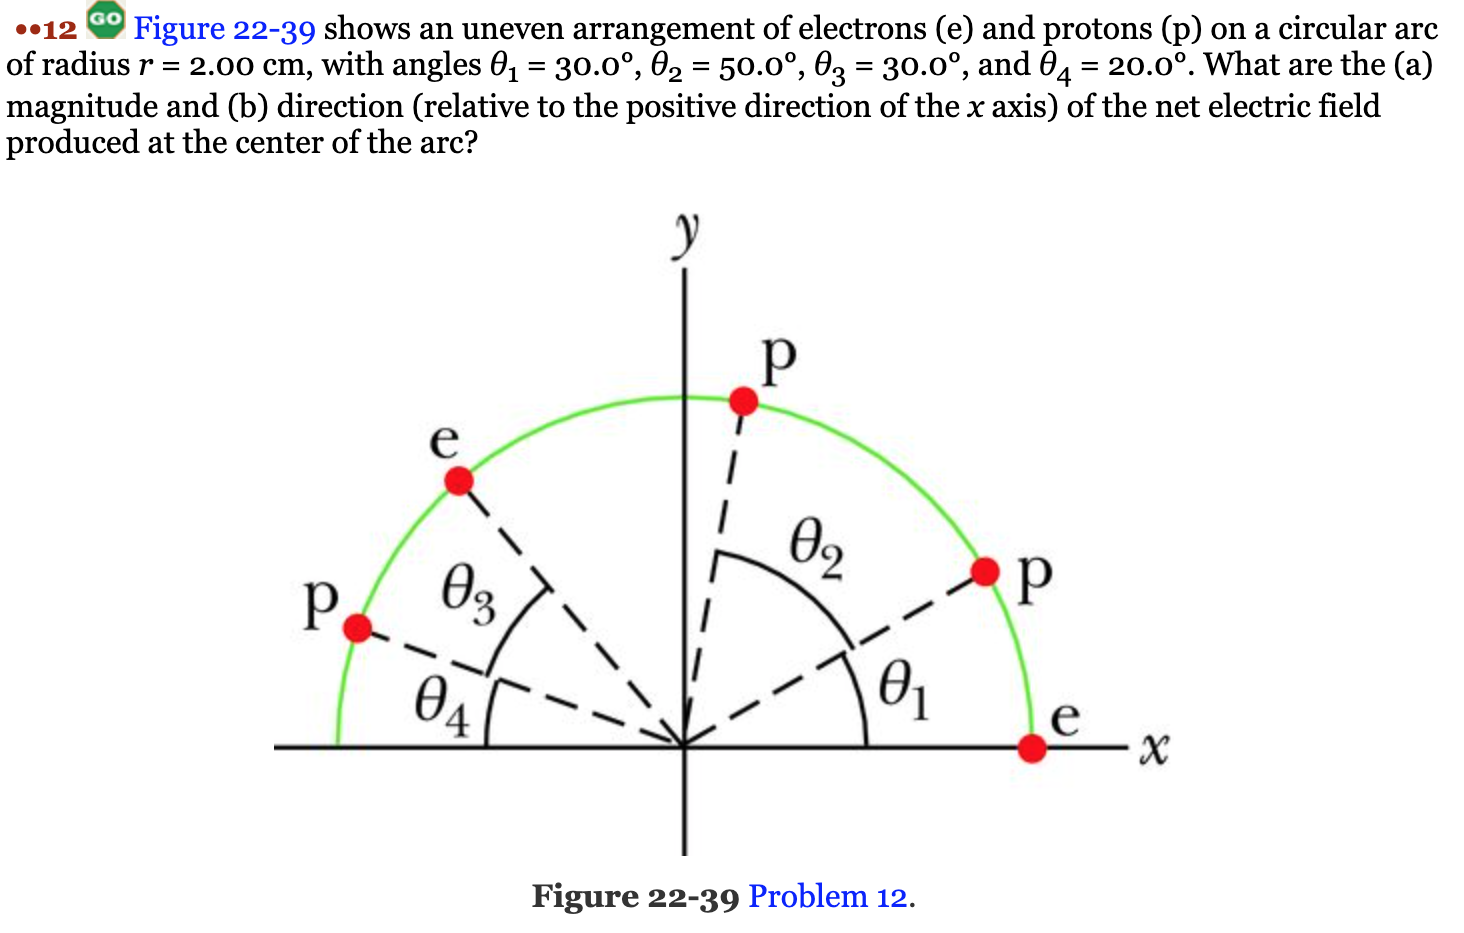
\includegraphics[width=\textwidth]{picture_6.png}


\pagebreak
\section*{Chapter 22, Problem 46}
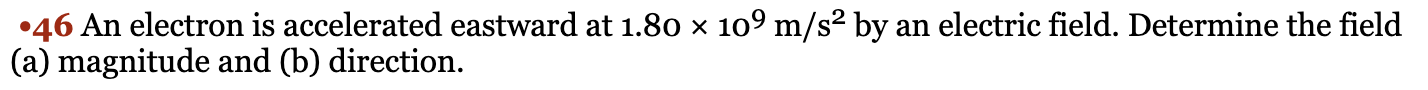
\includegraphics[width=\textwidth]{picture_7.png}

\subsection*{Solution}
The formula we have from Newton's second law is $\vec{F}_{net} = m\vec{a}$. We already have the acceleration, that being $1.80 \times 10^9 \unit{\meter/\second^2}$ eastward. We can also apply the mass of the electron ($9.1093837 \times 10^{-31} \unit{\kilo\gram}$), also keeping in mind the charge of an electron ($-1.60217663 \times 10^{-19} \unit{\coulomb}$). We can also keep in mind that $\vec{F}_{net} = q \vec{E}_{net}$
\begin{align*}
    \vec{F}_{net}   =   m\vec{a}
        &=  q \vec{E}_{net}\\
    \vec{E}_{net}   &=  \frac{m\vec{a}}{q}
        =   \frac{(9.1093837 \times 10^{-31} \unit{\kilo\gram})*(1.80 \times 10^9 \unit{\meter/\second^2})}{-1.60217663 \times 10^{-19} \unit{\coulomb}}\\
        &=  -1.02341342103 \times 10^{-2} \unit{\newton/\coulomb}
\end{align*}

a) Since we are looking for the magnitude, we take the absolute value, which is (approximately) \boxed{1.0234 \times 10^{-2} \unit{\newton/\coulomb}}.

b) Since the original charge was going eastward and the electric field is in the opposite direction, the direction is \boxed{\text{westward}}.

\end{document}